\documentclass[preprintnumbers,amsmath,amssymb,onecolumn,12pt]{revtex4}
\usepackage{graphicx}% Include figure files
\usepackage{dcolumn}% Align table columns on decimal point
\usepackage{bm}% bold math
\usepackage{natbib}
\usepackage[caption=false]{subfig}

\def\sgn{\mathop{\rm sgn}}

\begin{document}

\vspace{0.2in}
{\Large \hspace{1.6in}\textsc{Supplementary Material} }\\
\
\title{Mechanical Detection of Dipole-Dipole Interactions \\between Electronic Spins in a Solid}

\author{C. Pellet-Mary, P. Huillery, M. Perdriat, G. H\'etet} 


\affiliation{$^1$
Laboratoire de Physique de l'Ecole normale sup\'erieure, ENS, Universit\'e PSL, CNRS, Sorbonne Universit\'e, Universit\'e Paris-Diderot, Sorbonne Paris Cit\'e, Paris, France.
}

\begin{abstract}
\end{abstract}

\maketitle

\tableofcontents

\newpage

\section*{Experimental details}

\subsection{Experimental setup}

As illustrated in Fig.\ref{Optics}, the diamond sample is typically illuminated with 1mW of 532 nm laser light, focused by a NA = 0.5 objective. An acousto-optic modulator (AOM) is used to switch on and off the 532nm laser and to finely tuned its power. The photo-luminescence (PL) is collected by the objective, separated form the excitation light using a dichroic mirror (DM) and a 532nm notch filter (NF), and detected using a multimode-fibered single-photon avalanche photo-detector (APD) (SPCM-AQRH-15 from Perkin Elmer). Typically, we detect PL photons at a rate of 1MHz. 

\begin{figure}[!ht]
  \centering \scalebox{0.7}{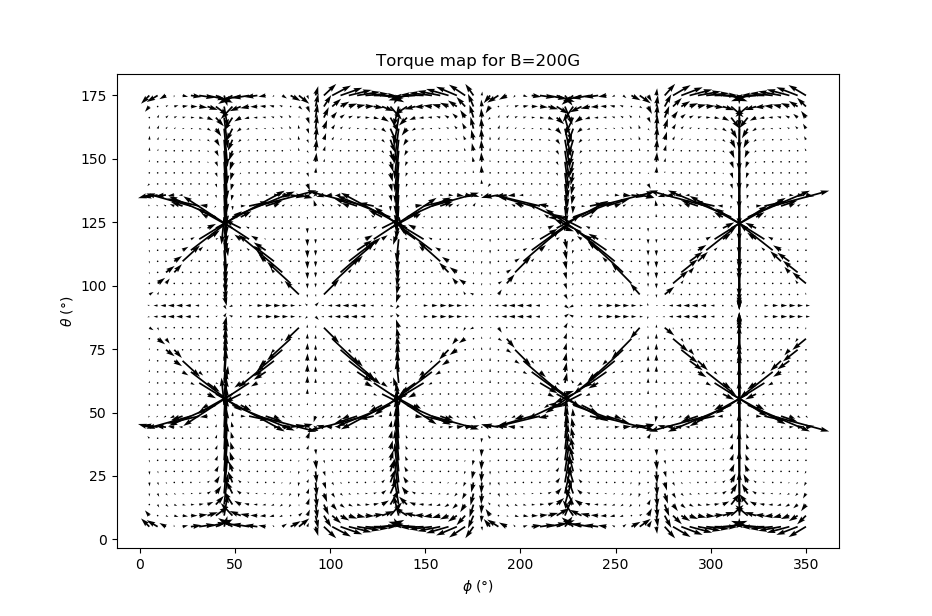
\includegraphics{map_200G_juste_CR}}
  \caption{?}
	\label{Optics}
\end{figure}

\begin{figure}[!ht]
  \centering \scalebox{0.7}{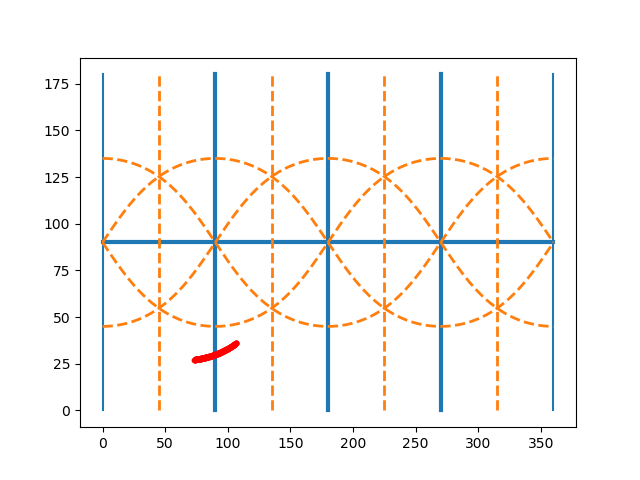
\includegraphics{map_cross_22}}
  \caption{?}
	\label{Optics}
\end{figure}


\begin{figure}[!ht]
  \centering \scalebox{0.7}{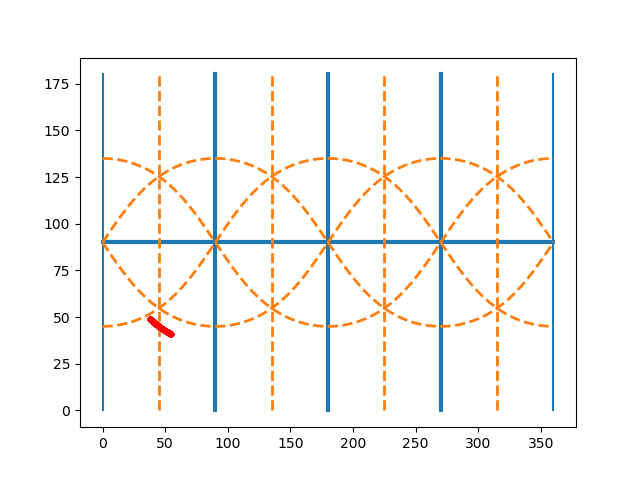
\includegraphics{map_cross_121}}
  \caption{?}
	\label{Optics}
\end{figure}

\begin{figure}[!ht]
  \centering \scalebox{0.5}{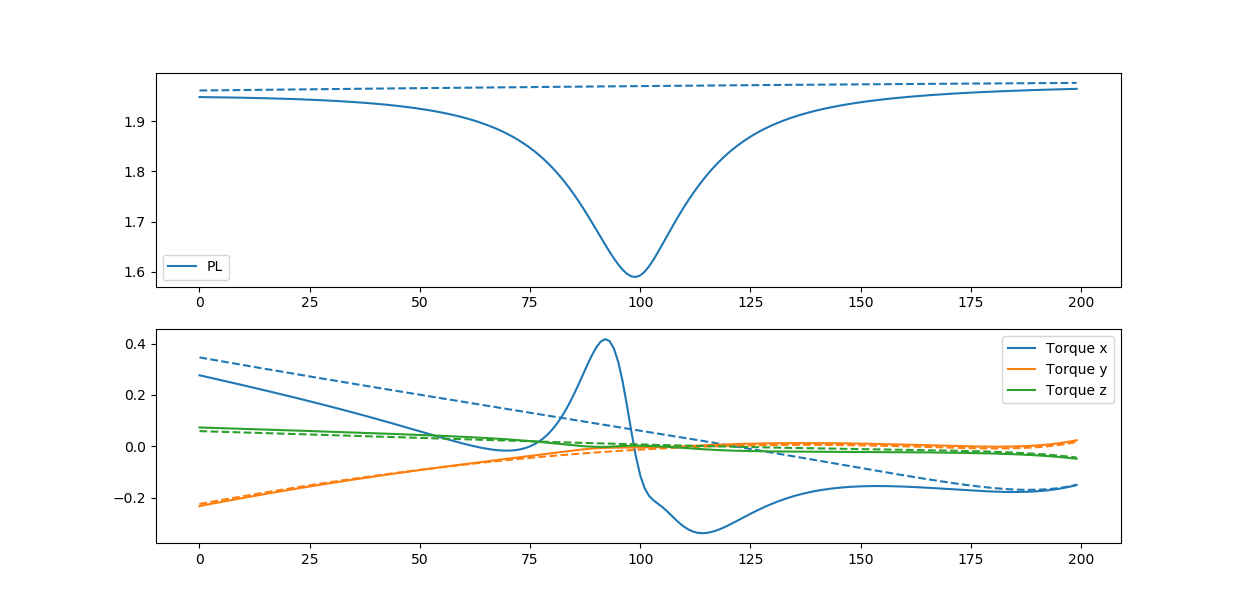
\includegraphics{cross_22_200G}}
  \caption{?}
	\label{Optics}
\end{figure}

\subsection{$T_1$ Measurement}
%Include graphics...
The protocol to measure the spin lifetime of the NV centers is described in Fig. ... . The spins are initially polarized in their $m_s=\ket{0}$ state through a 1 ms green laser excitation pulse and then left to evolove in the dark for a variable dark time $\tau$. The spin state is finally read out with a 10 $\mu$s laser pulse, shorter than the polarization time of the spins.

The sequence is repeated a second time, adding a resonnant microwave $\pi$ pulse on a transition of one of the four classes of NV$^-$, exchanging the population of the $m_s=\ket{0}$ state with one of the $m_s=\ket{\pm 1}$ state.

The two sequences are then substracted, allowing us to measure the spin state population of a single class, and removing unwanted constributions such as charge state transfer in the dark.

\subsection{Magnetic field calibration}

A permanent magnet is placed a few cm away from the diamond sample in order to apply a uniform magnetic field to the NV centers together with an electro-magnet.

To calibrate the magnetic field magnitude $B$, and its orientation $\theta$ with respect to the NV axis, we record Optically Detected Magnetic Resonace (ODMR) spectra.... 



\subsection{Spin-mechanical detection}

The microwave detuning is scanned in 2~MHz steps with a duration of 10 ms per points. During those 10ms, the diamond orientation has enough time to reach its equilibrium position and the spin torque effect can be observed. The average count-rate is about 1 MCounts/s.

\subsection{PL detection}

In these measurements, compared to \cite{DelordNat}, to detect the PL we use another detection channel that is more resilient to motion. We therefore do not need to detect prior to ring down.


\bibliography{Bib-with-NV-Nuclear-spins}

\end{document}
